%Trabajo Fin de Grado en Matematicas curso 2025-26
%version 2025-10-02
\documentclass[vecarrow,envcountsame,envcountchap,oribibl]{svmono}
\usepackage[spanish]{babel} \decimalpoint
\usepackage[latin1]{inputenc}


\usepackage{amsmath}
\usepackage{amssymb}
\usepackage{makeidx}
\usepackage{multicol}
\usepackage[a4paper]{geometry}
\usepackage[file]{smtfg}
   %\usepackage{smtfg} para mostrar hipervínculos en negro (compilar para imprimir en papel)
   %\usepackage[file]{smtfg} para mostrar hipervínculos en azul (compilar para crear fichero .pdf optimizado para navegación)

\smartqed
% para indentar a la derecha el símbolo de final de demostración (este comando viene definido en el fichero clase svmono.cls)

\makeindex

%%%%%%%%%%%%%%%%%%%%%%%%%%%%%%%%%%%%%%%%%%%%%%%%%%%%%%%%%%%%%%%%%%%%%%%%%%%%%%%
%%%%%%%%%%%%%%%%%%%  propiedades del fichero pdf  %%%%%%%%%%%%%%%%%%%%%%%%%%%%%
%%%%%%%%%%%%%%%%%%%%%%%%%%%%%%%%%%%%%%%%%%%%%%%%%%%%%%%%%%%%%%%%%%%%%%%%%%%%%%%
\hypersetup{%
   pdftitle={Como se titule este Trabajo Fin de Grado},
   pdfauthor={Autor del TFG},
   pdfsubject={Línea del TFG}, 
   pdfkeywords={Palabras Clave}
}

%%%%%%%%%%%%%%%%%%%%%%%%%%%%%%%%%%%%%%%%%%%%%%%%%%%%%%%%%%%%%%%%%%%%%%%%%%%%%%%
%%%%%%%%%%%%%%%%%%%  tutores  %%%%%%%%%%%%%%%%%%%%%%%%%%%%%%%%%%%%%%%%%%%%%%%%%
%%%%%%%%%%%%%%%%%%%%%%%%%%%%%%%%%%%%%%%%%%%%%%%%%%%%%%%%%%%%%%%%%%%%%%%%%%%%%%%

\PT{Nombre del Primer Tutor}
\InsPT{Universidad de La Laguna\\
38200 La Laguna, Tenerife}
\DptoPT{Departamento del Primer TutorQueEsLargo}
\EmPT{email1Tutor@ull.es}

\ST{Nombre del Segundo Tutor}
\InsST{Universidad de La Laguna\\
38200 La Laguna, Tenerife}
\DptoST{Departamento del Segundo Tutor}
\EmST{email2Tutor@ull.es}

\CONV{mes}{a\~no}

%%%%%%%%%%%%%%%%%%%%%%%%%%%%%%%%%%%%%%%%%%%%%%%%%%%%%%%%%%%%%%%%%%%%%%%%%%%%%%%
%%%%%%%%%%%%%%%%%%%   comandos personales   %%%%%%%%%%%%%%%%%%%%%%%%%%%%%%%%%%%
%%%%%%%%%%%%%%%%%%%%%%%%%%%%%%%%%%%%%%%%%%%%%%%%%%%%%%%%%%%%%%%%%%%%%%%%%%%%%%%
% define an unnumbered environment 
\spnewtheorem*{prop}{Propiedades}{\itshape}{\rmfamily}

% mycommands.tex contiene los comandos (atajos) particulares para el autor
% añade en mycommmands.tex los que quieras
%%%%%%%%%%%%%%%%%%%%%%%%%%%%%%%%%%%%%%%%%%%%%%%%%%%%%%%%%%%%%%%%%%%%%%%%%%%%%%%%
%%%%%%%%%%%%%%%%%%%%%%%%%%                               %%%%%%%%%%%%%%%%%%%%%%%
%%%%%%%%%%%%%%%%%%%%%%%%%%    NEW MATH OPERATORS         %%%%%%%%%%%%%%%%%%%%%%%
%%%%%%%%%%%%%%%%%%%%%%%%%%                               %%%%%%%%%%%%%%%%%%%%%%%
%%%%%%%%%%%%%%%%%%%%%%%%%%%%%%%%%%%%%%%%%%%%%%%%%%%%%%%%%%%%%%%%%%%%%%%%%%%%%%%%

\DeclareMathOperator{\sop}{\mathrm{sop}}
\DeclareMathOperator{\dist}{\mathrm{dist}}
\DeclareMathOperator{\diam}{\mathrm{diam}}
\DeclareMathOperator{\lon}{\mathrm{long}}



%%%%%%%%%%%%%%%%%%%%%%%%%%%%%%%%%%%%%%%%%%%%%%%%%%%%%%%%%%%%%%%%%%%%%%%%%%%%%%%%
%%%%%%%%%%%%%%%%%%%%%%%%                                %%%%%%%%%%%%%%%%%%%%%%%%
%%%%%%%%%%%%%%%%%%%%%%%%  NUEVOS COMANDOS MATEMÁTICOS   %%%%%%%%%%%%%%%%%%%%%%%%
%%%%%%%%%%%%%%%%%%%%%%%%                                %%%%%%%%%%%%%%%%%%%%%%%%
%%%%%%%%%%%%%%%%%%%%%%%%%%%%%%%%%%%%%%%%%%%%%%%%%%%%%%%%%%%%%%%%%%%%%%%%%%%%%%%%

\newcommand\orint{\ensuremath{\varointctrclockwise}}
\newcommand\mf[1]{\ensuremath{\mathfrak{#1}}}
\newcommand\cg[1]{\ensuremath{\mathcal{#1}}}
\newcommand\bs[1]{\ensuremath{\boldsymbol{#1}}}
\newcommand\mc[1]{\ensuremath{\mathcal{#1}}}
\newcommand\mb[1]{\ensuremath{\mathbb{#1}}}
\newcommand\C{\ensuremath{\mathbb{C}}}
\newcommand\R{\ensuremath{\mathbb{R}}}
\newcommand\Z{\ensuremath{\mathbb{Z}}}
\newcommand\U{\ensuremath{\mathbb{D}}}
\newcommand\ve{\ensuremath{\varepsilon}}
\newcommand\vr{\ensuremath{\varrho}}
\newcommand\ds{\displaystyle}
\newcommand\p[1]{\ensuremath{\partial #1}}
\newcommand\dn[1]{\ensuremath{\partial\sb{\vec{n}}#1\,}}
\newcommand\nd[1]{\ensuremath{\partial\sb{\vec{n}\sb#1}}}

\newcommand{\din}{\ensuremath{\mathbin{\rotatebox[origin=c]{-90}{$\in$}}}}
\newcommand{\upar}{\ensuremath{\mathbin{\rotatebox[origin=c]{90}{$)$}}}}

\makeatletter
\newcommand*{\subsetsim}{%
  \mathrel{%
    \mathchoice
    {\@subsetsim\displaystyle\scriptstyle}%
    {\@subsetsim\textstyle\scriptstyle}%
    {\@subsetsim\scriptstyle\scriptscriptstyle}%
    {\@subsetsim\scriptscriptstyle\scriptscriptstyle}%
  }%
}
\newcommand*{\@subsetsim}[2]{%
  \sbox0{$\m@th#1\subset$}%
  \sbox2{$\m@th#2\sim$}%
  \sbox4{$\m@th#2$}%
  \raisebox{.5\dimexpr\ht2-\ht4\relax}{%
    \oalign{\copy0 \cr\hidewidth\copy2\hidewidth}%
  }%
}



%%%%%%%%%%%%%%%%%%%%%%%%%%%%%%%%%%%%%%%%%%%%%%%%%%%%%%%%%%%%%%%%%%%%%%%%%%%%%%%%
%%%%%%%%%%%%%%%%%%%%%%%%%%                               %%%%%%%%%%%%%%%%%%%%%%%
%%%%%%%%%%%%%%%%%%%%%%%%%%  NUEVOS ENTORNOS MATEMÁTICOS  %%%%%%%%%%%%%%%%%%%%%%%
%%%%%%%%%%%%%%%%%%%%%%%%%%                               %%%%%%%%%%%%%%%%%%%%%%%
%%%%%%%%%%%%%%%%%%%%%%%%%%%%%%%%%%%%%%%%%%%%%%%%%%%%%%%%%%%%%%%%%%%%%%%%%%%%%%%%
% define some unnumbered environments 
\spnewtheorem*{nota}{Nota:}{\slshape}{\rmfamily}
\spnewtheorem*{snota}{Nota}{\slshape}{\rmfamily}
\spnewtheorem*{pf}{Demostración.}{\itshape}{\rmfamily}
  



%%%%%%%%%%%%%%%%%%%%%%%%%%%%%%%%%%%%%%%%%%%%%%%%%%%%%%%%%%%%%%%%%%%%%%%%%%%%%%%
%%%%%%%%%%%%%%%%%%%     documento     %%%%%%%%%%%%%%%%%%%%%%%%%%%%%%%%%%%%%%%%%
%%%%%%%%%%%%%%%%%%%%%%%%%%%%%%%%%%%%%%%%%%%%%%%%%%%%%%%%%%%%%%%%%%%%%%%%%%%%%%%


\includeonly{./frontmatter/ack,./frontmatter/res,./frontmatter/intro,./mainmatter/chap1,./mainmatter/chap2,./mainmatter/conclusiones,./mainmatter/app,./backmatter/biblio,./backmatter/acron}

%Si solo queremos procesar el segundo capítulo, pero conservando todas las referencias que se hayan utilizado en las otras partes...
%\includeonly{./mainmatter/chap2}
%lo que producirá un pdf con la portada, el índice y el capítulo 2 únicamente




\begin{document}\allowdisplaybreaks

\author{Autor del TFG}
\EmAut{emailAuTFG@ull.edu.es}
\title{\slshape T\'{\i}tulo de este trabajo fin de grado}
\subtitle{Subtitle in English of this dissertation}

\pdfbookmark[-1,bold,italic]{Título del TFG}{title}
\maketitle

\frontmatter


\bookmarksetup{bold,color=blue!150}
\ack



Quiero agradecer a mis pies por apoyarme en todo momento y a mis brazos por estar siempre a mi lado. Y c\'omo olvidar a mis dedos con quienes siempre puedo contar.


\vfil
\begin{flushright}
\hfill Autor del TFG\\
La Laguna, \today
\end{flushright}

\clearemptydoublepage
\bookmarksetup{bold=false,color={},color=blue}
\abs
\vspace*{-1.5cm}

\begin{resumen}
Resumen en espa\~nol. Escribir un buen resumen es una tarea dif\'{\i}cil que solo puede
realizarse tras haber finalizado la escritura del trabajo. Ha de resumir los resultados
de la investigaci\'on permitiendo al lector hacerse una idea del trabajo sin que necesite
leerlo por completo. Tras leer el resumen otros investigadores deben ser capaces de
decidir si vale la pena leer el trabajo. Debe proporcionar informaci\'on suficiente
sobre los objetivos y logros del trabajo, y tal vez sobre las t\'ecnicas y herramientas
utilizadas.

Evita en la medida de lo posible notaci\'on matem\'atica en el resumen. Si es
imprescindible que aparezca una referencia bibliogr\'afica ha de ponerse entera:
el resumen debe ser una pieza de texto independiente, pues puede aparecer publicada
en otros documentos, bases de datos, websites, etc. Ten en cuenta que el resumen es la
parte de tu trabajo que m\'as gente va a leer. Merece la pena dedicarle
la atenci\'on necesaria.
\palabrasclave{Palabra clave 1 -- Palabra clave 2 --Palabra clave 3 -- $\ldots$.}
\end{resumen}

\vfil

\begin{abstract}
Abstract in English.
A good abstract is
difficult to write and can only be completed after the full dissertation has been
written. It represents a brief summary of the results of the dissertation research. By
summarising the results of the research, it allows other people to get an idea of what
was accomplished without having to read through the whole dissertation. Other
scholars can read an abstract to decide if looking at the full work will be worthwhile.
The abstract should provide sufficient information about the results of the research
that reading the full dissertation is not necessary, although your markers will read the
full dissertation. (\dots)
\keywords{Keyword 1 -- Keyword 2 -- Keyword 3 -- $\ldots$.}

\end{abstract}

\clearemptydoublepage

\pdfbookmark[-1,bold,color=brown!200]{\contentsname}{Contents}
\tableofcontents
\bookmarksetup{bold=false,color=magenta}
  \intro


Aqu\'{\i} la introducci\'on del trabajo. En \cite{guidedissertation} pueden leerse
estos consejos:

The dissertation should be divided into chapters and sections appropriate to
the topic and type of dissertation chosen. The following elements are typical
of the traditional dissertation. You should discuss the overall structure of
your dissertation with your academic supervisor.

The Introduction to the dissertation should set out the background to the
research study and address the following areas:

\medskip
\noindent\textsl{The context in which the research took place}
\begin{itemize}
 \item What is the background, the context, in which the research took place?
 \item Why is this subject or issue important?
 \item Who are the key participants and/or `actors' in the area under investigation?
 \item Are there important trends or pivotal variables of which the reader
       needs to be made aware?
 \item A clear and succinct statement of the aims and objectives that the
       dissertation is going to address.
 \item Have you presented a clear and unambiguous exposition of your research
       aim, the objectives you will address to meet this aim and your research
       questions?
\end{itemize}

\medskip
\noindent\textsl{The reasons why this study was carried out}
\begin{itemize}
 \item Was this study undertaken for example in order to test some aspect of
professional or business practice or theory or framework of analysis?
 \item Was the research carried out to fulfil the demands of a business
organisation?
\end{itemize}

\medskip
\noindent\textsl{The way the Dissertation is to be organised}

You should write your dissertation with the idea in mind that the intended reader and
reviewer has some shared understanding of the area being investigated, however,
underpinning concepts and arguments still need to be included as otherwise the depth
of research will be compromised. In this way, you will not be tempted to make too
many implicit assumptions, i.e. by making the erroneous assumptions that the reader
has your degree of knowledge about the matters in question or can follow, exactly,
your thought processes without your spelling them out. It should be a document which
is `self-contained' and does not need any additional explanation, or interpretation, or
reference to other documents in order that it may be fully understood.

This short final section of the Introduction should tell the reader what topics are going
to be discussed in each of the chapters and how the chapters are related to each other.
In this way, you are, in effect, providing the reader with a `road map' of the work
ahead. Thus, at a glance, they can see (1) where they are starting from, (2) the context
in which the journey is taking place, (3) where they are going to end up, and (4) the
route which they will take to reach their final destination. Such a `map' will enable
the reader to navigate their way through your work much more easily and appreciate
to the maximum what you have done.

    
\clearemptydoublepage

\mainmatter
\bookmarksetup{bold=false,color={},color=blue}
\chapter{T\'{\i}tulo del primer cap\'{\i}tulo}\label{chap:fundamentos}

Each of your chapters will require both an introduction and a conclusion. The former
provides the reader with a contents `map' of what is to come, and the latter provides a
concise summary of what they have just read. 

\section{Primera Secci\'on}
Each introduction should look back to
the conclusion of the previous chapter, and forwards to the contents of the chapter
which you are introducing. The conclusion should look back into the chapter just
completed, and forward to the introduction of the following chapter. These
conclusions and introductions act like small links which bind the `chain' of the
chapters together in a more seamless whole than would have occurred if the chapters
had not been introduced or concluded; they `smooth out'  the transition from chapter
to chapter and from topic to topic. (Tomado de \cite{guidedissertation}.)


\subsection{Primera sub-secci\'on de la Primera Secci\'on}
\label{subsec:unaparaempezar}
Algo de texto y una gr\'afica para ver esta primera subsecci\'on.
\begin{figure}
  \begin{center}
   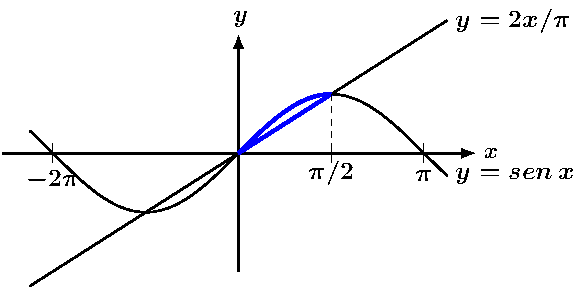
\includegraphics[scale=0.8]{./ilustraciones/fig1.pdf}
   \end{center}
   \caption{Una gr\'afica siempre viene bien para ilustrar el texto.}
   \label{fig:ejemplografica}
\end{figure}

No siempre aparecen las figuras (y las tablas) en el lugar exacto donde se
ponen en el archivo .tex. Aunque se tiene un cierto control sobre ello con los par\'ametros, al final es \LaTeX{} quien decide d\'onde ponerla.

Tambi\'en puede ser \'util poner tablas.
\begin{table}
\begin{center}
   \begin{tabular}{ r @{\hspace{1.3em}} r @{\hspace{1em}} r r }
       \textbf{A\;} & \textbf{B\;} & \textbf{C\;} & \textbf{Resto} \\
       \hline\noalign{\smallskip} 
       44.2 & 5.1 & 6.1 & 2.3\\
       712.2 & 8.3 & 99.2 & 3.1\\
       \hline
   \end{tabular}
   \caption{\label{tab:pocoutil}
   Una tabla peque\~na pero in\'util. Bueno, al menos es peque\~na, \textquestiondown no?}
\end{center}
\end{table}

Puedo referirme m\'as tarde tanto a la figura~\ref{fig:ejemplografica} de la p\'agina~\pageref{fig:ejemplografica}
como a la tabla~\ref{tab:pocoutil} de la p\'agina~\pageref{tab:pocoutil}, ambas
de la la subsecci\'on~\ref{subsec:unaparaempezar}. Para ello utilizamos los
comandos \verb$\label$ \verb$\ref$ y \verb$\pageref$



\section{Segunda Secci\'on}
Primero definimos lo que es un \emph{matem\'atico}, ese ser rarito y ensimismado.
\begin{definition}[Paul Erd\H os]
  Un \emph{matem\'atico} es un dispositivo que convierte caf\'e en teoremas.
\end{definition}
\begin{conjecture}
Me parece que se me va a olvidar todo esto.
\end{conjecture}
\begin{corollary}
Para qu\'e me lo voy a aprender.
\end{corollary}

\subsection{Primera sub-secci\'on de la Segunda Secci\'on}

\subsubsection{Primera sub-sub-secci\'on de la Primera subsecci\'on de la Segunda Secci\'on}
\begin{itemize}
  \item primer elemento de la lista
  \item este es el segundo
  \item y hay un tercero que se divide
  \begin{itemize}
    \item primera subdivisi\'on
    \item segundo tipo del tercer elemento
  \end{itemize}
\end{itemize}

Conviene tener en cuenta que al combinar los distintos atributos en las fuentes
de texto, no siempre resulta lo esperado:
\begin{center}
\begin{tabular}{cccccc}
      &    &\small\verb;\upshape; & \small\verb;\itshape;
           &\small\verb;\slshape; & \small\verb;\scshape;\\
\cline{2-6}
\small\verb;\rmfamily; & \small\verb;md; &
  \rmfamily\mdseries\textup{vertical} &
  \rmfamily\mdseries\textit{it\'alica}&
  \rmfamily\mdseries\textsl{inclinada}&
  \rmfamily\mdseries\textsc{Versalita}\\
      & \small\verb;bf; &
  \rmfamily\bfseries\textup{vertical} &
  \rmfamily\bfseries\textit{it\'alica}&
  \rmfamily\bfseries\textsl{inclinada}&
  \rmfamily\bfseries\textsc{Versalita}\\
\cline{2-6}
\small\verb;\sffamily; & \small\verb;md; &
  \sffamily\mdseries\textup{vertical} &
  \sffamily\mdseries\textit{it\'alica}&
  \sffamily\mdseries\textsl{inclinada}&
  \sffamily\mdseries\textsc{Versalita}\\
      & \small\verb;bf; &
  \sffamily\bfseries\textup{vertical} &
  \sffamily\bfseries\textit{it\'alica}&
  \sffamily\bfseries\textsl{inclinada}&
  \sffamily\bfseries\textsc{Versalita}\\
\cline{2-6}
\small\verb;\ttfamily; & \small\verb;md; &
  \ttfamily\mdseries\textup{vertical} &
  \ttfamily\mdseries\textit{it\'alica}&
  \ttfamily\mdseries\textsl{inclinada}&
  \ttfamily\mdseries\textsc{Versalita}\\
      & \small\verb;bf; &
  \ttfamily\bfseries\textup{vertical} &
  \ttfamily\bfseries\textit{it\'alica}&
  \ttfamily\bfseries\textsl{inclinada}&
  \ttfamily\bfseries\textsc{Versalita}\\
\cline{2-6}
\end{tabular}
\end{center}


\clearpage
\chapter{Segundo Cap\'{\i}tulo}
En el cap\'{\i}tulo \ref{chap:fundamentos} pudimos ver un interesante ejemplo
del uso de referencias y numeraci\'on de elementos que nos permite referirnos a la
gr\'afica de la figura \ref{fig:ejemplografica} de la p\'agina
\pageref{fig:ejemplografica}.


\section{Primera secci\'on}
\subsection{Primera subsecci\'on de la Primera secci\'on}
\subsubsection{Segunda subsubsecci\'on de la Primera secci\'on}



\subsection{Segunda subsecci\'on de la Primera secci\'on}
\subsection{Tercera subsecci\'on  de la Primera secci\'on}
\subsubsection{Primera subsubsecci\'on de la tercera subsecci\'on de la Primera secci\'on}


%\clearpage
%\include{./mainmatter/chap3}
%\clearpage
%\include{./mainmatter/chap4}
\clearpage
\chapter*{Conclusiones}

De nuevo unos sabios consejos tomados de \cite{guidedissertation}: \\
Here you will bring together the work of the dissertation by showing how the
initial research plan has been addressed in such a way that conclusions may be
formed from the evidence of the dissertation. No new material or references
should be placed here. The conclusions should make a statement on the extent
to which each of the aims and objectives has been met. You should bring back
your research questions and state clearly your understanding of those questions.
Be careful not to make claims that are not substantiated from the evidence you
have presented in earlier chapters.

If you are undertaking a company project based around a business issue do not
confuse recommendations for the company with conclusions. If you want to
include a list of recommendations then do so in a separate short chapter.
\emph{The conclusions address the wider understanding of the issue you have
been studying.}

You should include a short sub section on any suggestions for further research
for colleagues who might wish to undertake research in this area in the future.
There should also be a short statement of the limitations of the research. Often
as a single case study or limited range of companies you can not really claim
that your research holds for all companies. However, by adopting a rigorous
approach to your literature review and methods which have validity and can be
repeated you can make a reasonable but limited claim that your conclusions
should be taken seriously.



\appendix
\chapter{Ap\'endice}

\section{Primera secci\'on del Ap\'endice}
\subsection{Primera sub-secci\'on de la Primera secci\'on del Ap\'endice}


\backmatter

\bookmarksetup{color=bibcolor}
\phantomsection
\addcontentsline{toc}{chapter}{Bibliografía}







\begin{thebibliography}{99}

\bibitem[$\blacktriangleright$]{intro}
Citar las fuentes que hayas utilizado no es solo una cuesti\'on de honradez personal sino tambi\'en de justicia con los autores de los que te has ayudado. No citar propiamente es apropiarse del trabajo y m\'erito ajeno y podr\'{\i}a considerarse plagio.

\medskip
Las referencias bibliogr\'aficas deben seguir un formato coherente. Elige el que quieras (puedes consultar \cite{bbtkULLcitas} para ver algunos), lo importante es que ofrezcas todos los datos para localizar la referencia. Tambi\'en debes citar los recursos de la red que hayas utilizado as\'{\i} como el \textsl{software}.

\medskip
Siguiendo la norma UNE 50-104-94 (adaptaci\'on espa\~nola de la ISO 690) las distintas referencias a libros, cap\'{\i}tulos de libro, art\'{\i}culos en revistas o documentos en internet quedar\'{\i}an tal como se muestra:
\bigskip


%libro. El título en cursiva
\bibitem{latexbook} LAMPORT, Leslie. 
\emph{\LaTeX: A Document Preparation System, User's Guide and Reference Manual.} 2nd edition.
Reading: Addison-Wesley, 1994. 


%libro en internet
\bibitem{latexwiki}  
\emph{\LaTeX} [en l\'{\i}nea].
WikiBooks. [Consulta: 17-10-2019] Disponible en: \url{https://en.wikibooks.org/wiki/LaTeX}.


%capitulo de un libro (cada capítulo tiene autores diferentes)
\bibitem{autorias}
MOSTELLER, F. y WALLACE, D.L.
Decisi\'on de autor\'{\i}as.
En TANUR, J.M., MOSTELLER, F., KRUSKAL, W.H., LEHMANN, E.L., LINK, R.F., PIETERS, R.S. y RISING, G.R. (editores)
\emph{La Estad\'{\i}stica: Una gu\'{\i}a de lo desconocido}.
Madrid: Alianza, 1992, pp. 187--200.


%revistas: el título de la revista en cursiva
\bibitem{wagner}
WAGNER, C.H. Simpson's Paradox in Real Life.
\emph{The American Statistician}, 1982, vol. 36, pp. 46--48.


%recurso en internet
\bibitem{bbtkULLcitas}
Biblioteca de la Universidad de La Laguna.
\emph{C\'omo citar la informaci\'on} [en l\'{\i}nea]. [Fecha de consulta: 2-10-2025].
Disponible en: \url{https://ull-es.libguides.com/guiaparacitar}.


\bibitem{guidedissertation}
School of Management \& Languages.
\emph{A Guide To Writing Your Masters Dissertation} [en l\'{\i}nea]. 2011.
Heriot Watt University, Reino Unido.
[Fecha de consulta: 2-10-2025].
Disponible en: \url{https://www.researchgate.net/file.PostFileLoader.html?id=5769c2a840485404cf385288&assetKey=AS:375547478724608@1466548904040}
y tambi\'en en: \url{https://www.academia.edu/36590417/School_of_Management_and_Languages}



%software
\bibitem{R}
R Core Team. 
\emph{R: A language and environment for statistical computing}.
2019.
R Foundation for Statistical Computing, Vienna, Austria.
\url{https://www.R-project.org/}.


\end{thebibliography} 


\bookmarksetup{color=ullv}
\acron
(Toda esta p\'agina es opcional. Ponla solo si te parece necesario y con la notaci\'on que hayas utilizado en tu trabajo. En caso contrario puedes comentar la l\'{\i}nea \verb|\acron
(Toda esta p\'agina es opcional. Ponla solo si te parece necesario y con la notaci\'on que hayas utilizado en tu trabajo. En caso contrario puedes comentar la l\'{\i}nea \verb|\acron
(Toda esta p\'agina es opcional. Ponla solo si te parece necesario y con la notaci\'on que hayas utilizado en tu trabajo. En caso contrario puedes comentar la l\'{\i}nea \verb|\include{./backmatter/acron}| del archivo principal y no aparecerá nada.)
\vspace{2cm}

\begin{glos}
  \gitem{$\mathbb{C}\sb\infty$}{Esfera de Riemann}

  \gitem{$\partial/\partial\bar z$}{Operador de Cauchy Riemann $\frac{\partial}{\partial\bar z}=\frac{1}{2}\left(\frac{\partial}{\partial x}+i\frac{\partial}{\partial y}\right)$}

  \gitem{$\mathbb{T}$}{Circunferencia unidad}

  \gitem{$C(X,\R)$}{Funciones reales en $X$}

  \gitem{$C(K)$}{Funciones complejas continuas en $K$}

  \gitem{$C\sb c(X)$}{Funciones continuas con soporte compacto en $X$}

  \gitem{$C\sb0(X)$}{Clausura uniforme de $C\sb c(X)$}

  \gitem{$\Delta$}{Operador de Laplace $\Delta=4\partial\sp2\partial z\partial\bar z$ $\big/$ disco unidad}

  \gitem{$\Delta(a,r)$}%
        {Disco abierto de centro $a\in\mathbb{C}$ y radio $r>0$}

  \gitem{$L\sp2\sb{loc}(\Omega)$}%
        {Funciones de cuadrado localmente integrable en $\Omega$}

  \gitem{$\mathcal{O}(\Omega)$}{Funciones holomorfas en $\Omega$}

  \gitem{$\mathcal{O}(K)$}{Funciones holomorfas en un entorno de $K$}

  \gitem{$\omega\sb f(\delta)$}{M\'odulo de continuidad de $f$}

  \gitem{$U\Subset\Omega$}%
        {$U$ relativamente compacto en $\Omega$ ($\overline{U}$ compacto y $\overline{U}\subset\Omega$)}

  \gitem{PL}{Problema lineal}

  \gitem{PNL}{Problema no lineal}
\end{glos} 
| del archivo principal y no aparecerá nada.)
\vspace{2cm}

\begin{glos}
  \gitem{$\mathbb{C}\sb\infty$}{Esfera de Riemann}

  \gitem{$\partial/\partial\bar z$}{Operador de Cauchy Riemann $\frac{\partial}{\partial\bar z}=\frac{1}{2}\left(\frac{\partial}{\partial x}+i\frac{\partial}{\partial y}\right)$}

  \gitem{$\mathbb{T}$}{Circunferencia unidad}

  \gitem{$C(X,\R)$}{Funciones reales en $X$}

  \gitem{$C(K)$}{Funciones complejas continuas en $K$}

  \gitem{$C\sb c(X)$}{Funciones continuas con soporte compacto en $X$}

  \gitem{$C\sb0(X)$}{Clausura uniforme de $C\sb c(X)$}

  \gitem{$\Delta$}{Operador de Laplace $\Delta=4\partial\sp2\partial z\partial\bar z$ $\big/$ disco unidad}

  \gitem{$\Delta(a,r)$}%
        {Disco abierto de centro $a\in\mathbb{C}$ y radio $r>0$}

  \gitem{$L\sp2\sb{loc}(\Omega)$}%
        {Funciones de cuadrado localmente integrable en $\Omega$}

  \gitem{$\mathcal{O}(\Omega)$}{Funciones holomorfas en $\Omega$}

  \gitem{$\mathcal{O}(K)$}{Funciones holomorfas en un entorno de $K$}

  \gitem{$\omega\sb f(\delta)$}{M\'odulo de continuidad de $f$}

  \gitem{$U\Subset\Omega$}%
        {$U$ relativamente compacto en $\Omega$ ($\overline{U}$ compacto y $\overline{U}\subset\Omega$)}

  \gitem{PL}{Problema lineal}

  \gitem{PNL}{Problema no lineal}
\end{glos} 
| del archivo principal y no aparecerá nada.)
\vspace{2cm}

\begin{glos}
  \gitem{$\mathbb{C}\sb\infty$}{Esfera de Riemann}

  \gitem{$\partial/\partial\bar z$}{Operador de Cauchy Riemann $\frac{\partial}{\partial\bar z}=\frac{1}{2}\left(\frac{\partial}{\partial x}+i\frac{\partial}{\partial y}\right)$}

  \gitem{$\mathbb{T}$}{Circunferencia unidad}

  \gitem{$C(X,\R)$}{Funciones reales en $X$}

  \gitem{$C(K)$}{Funciones complejas continuas en $K$}

  \gitem{$C\sb c(X)$}{Funciones continuas con soporte compacto en $X$}

  \gitem{$C\sb0(X)$}{Clausura uniforme de $C\sb c(X)$}

  \gitem{$\Delta$}{Operador de Laplace $\Delta=4\partial\sp2\partial z\partial\bar z$ $\big/$ disco unidad}

  \gitem{$\Delta(a,r)$}%
        {Disco abierto de centro $a\in\mathbb{C}$ y radio $r>0$}

  \gitem{$L\sp2\sb{loc}(\Omega)$}%
        {Funciones de cuadrado localmente integrable en $\Omega$}

  \gitem{$\mathcal{O}(\Omega)$}{Funciones holomorfas en $\Omega$}

  \gitem{$\mathcal{O}(K)$}{Funciones holomorfas en un entorno de $K$}

  \gitem{$\omega\sb f(\delta)$}{M\'odulo de continuidad de $f$}

  \gitem{$U\Subset\Omega$}%
        {$U$ relativamente compacto en $\Omega$ ($\overline{U}$ compacto y $\overline{U}\subset\Omega$)}

  \gitem{PL}{Problema lineal}

  \gitem{PNL}{Problema no lineal}
\end{glos} 


\bookmarksetup{color=ullv}
\printindex

\end{document} 
